\vspace{12pt}
\section{General Electrical Characteristics of Bulk Samples}

The typical heterogeneity that characterizes ceramic materials leads to a broad range of conductivity performance. The electrical response of virtually all of our bulk samples were consistent with what is expected of polycrystalline materials: either one or two arcs in the Nyquist plot of $Z'$ vs. $Z''$ as shown for a typical case in Figure \ref{fig:general:eis}. As indicated in the figure, the overall resistance, as extracted from the intercept of the arc with the $Z'$ axis changes with the temperature. The behavior seen is typical of thermally activated processes, where the conductivity increases with increasing temperature. It is critical to ascertain that any given impedance arc corresponds to a transport process in the bulk of the sample, as opposed to electrode interface impedance. This is accomplished by measuring the dependence of the arc characteristics with and without an applied DC bias voltage. Arcs that do not substantially change with the application of DC bias can be attributed to ionic and/or electronic transport in the bulk or grain boundaries of the sample, while arcs that exhibit changes with DC bias originate in the polarization region between metallic contacts and the ceramic material. Both arcs shown in Figure \ref{fig:general:eis} show essentially no changes with applied DC biases and are therefore safely ascribed to bulk transport processes. All subsequent impedance arcs reported in this dissertation, as well as the sample conductivity values extracted from the arcs, have been confirmed to originate from bulk transport.

\begin{figure}
\centering
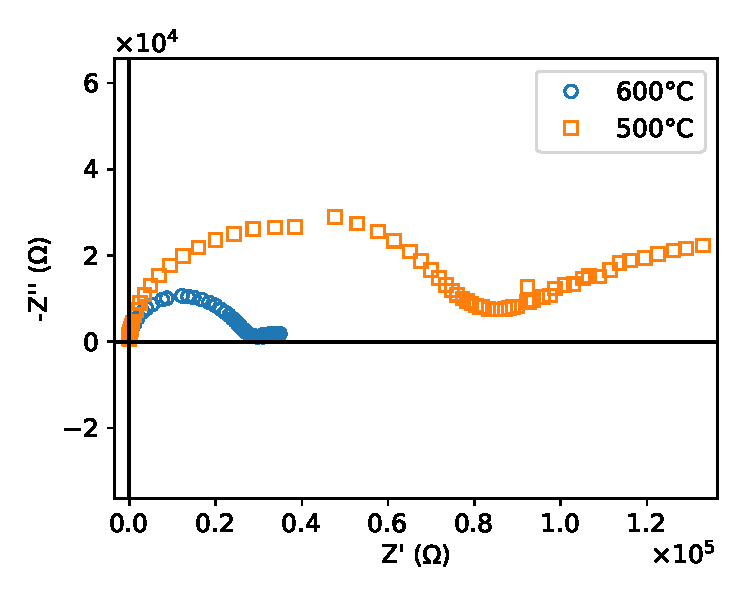
\includegraphics{Figures/171223-eis-bzg-pellet-dry-ar-two-temp-comparison.pdf}
 \caption{Typical impedance characteristics of a bulk sample measured at two different temperatures. A single bias-independent arc in the Nyquist plot is observed, indicating ionic transport. Data in this specific plots are from a Gd-doped barium zirconate bulk sample produced by solid state reaction with compensation for barium loss.}
 \label{fig:general:eis}
\end{figure}

\begin{figure}
\centering
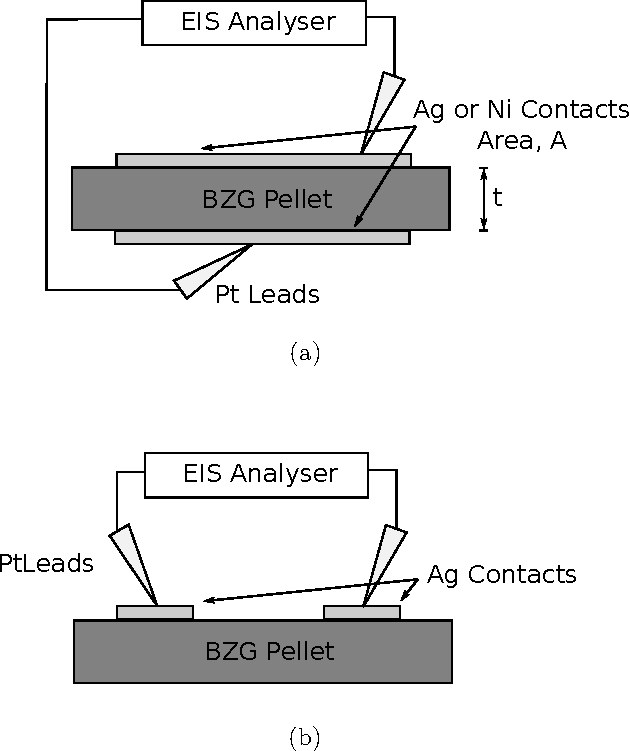
\includegraphics{Figures/bulkElectrodeGeometry.pdf}
  \caption{Geometry used for measuring the impedance of bulk samples. (a) ``Through-plane'' geometry. In this geometry the dimensions given can be used to determine the conductivity from the resistance by the standard formula. (b) ``In-plane'' geometry. This non-standard geometry prevents straightforward determination of conductivity, but comparisons of admittances (Y) can be made between samples of similar electrode geometry.}
  \label{fig:bulk:geometry}
\end{figure}

The impedance data exemplified by Figure \ref{fig:general:eis}, allows the study of the temperature dependence of the conductivity. An important element in extracting the conductivity from the impedance arcs is the taking into consideration of the measurement geometry. Figure \ref{fig:bulk:geometry}a shows the ``through-plane'' electrode geometry used in measuring bulk samples. The physical dimensions of our measurement electrode configuration yields a geometric factor that permits conversion of the resistance seen in the Nyquist to the needed conductivity. This is most effectively demonstrated by plotting the conductivity as a function of the inverse temperature ($T^{-1}$) in a standard Arrhenius plot as shown in Figure \ref{fig:general:arrhenius}. As described in the discussion leading to equation \ref{arrhenius}, the temperature dependence of the conductivity can be used to extract the activation energy of the conduction process. For bulk samples measured with ``in-plane'' electrode configuration shown in \ref{fig:bulk:geometry}b, the geometry does not lend itself to simple calculations of an effective geometrical constant and conductivity \cite{Jacobs1995}. However, since the conductivity is proportional to the admittance, Y, which is the inverse of resistance ($Y = 1/R$), comparison between these admittances at different temperatures can be made for samples of similar geometry. 

\begin{figure}
\centering
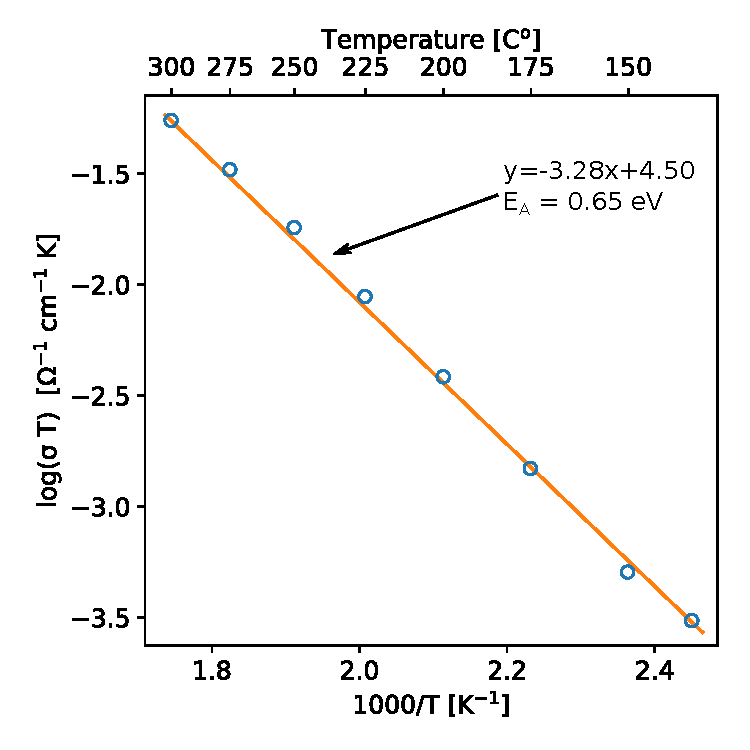
\includegraphics{Figures/170715-bzgxs10-pellet-thr-plane-air-edit.pdf}
  \caption{Arrhenius plot showing the temperature dependence of the conductivity of a bulk sample. Data in this specific plot is from a Gd-doped barium zirconate bulk sample produced by solid state reaction.}
  \label{fig:general:arrhenius}
\end{figure}
